% template adapted from https://github.com/jgm/pandoc-templates/blob/master/default.latex
%%%%%%%%%%%%%%%%%%%%%%%%%%%%%%%%%%%%%%%%%%%%%%%%%%%%%%%%%%%%%%%%%%%%%%%%%%%%%%%%%%%%%%%%%

% Options for packages loaded elsewhere
\PassOptionsToPackage{unicode=true}{hyperref}
\PassOptionsToPackage{hyphens}{url}
  \PassOptionsToPackage{dvipsnames,svgnames*,x11names*}{xcolor}


\documentclass[
  11pt,
  french,
  A4paper,
  extrafontsizes,onecolumn,openright
  ]{memoir}

% Font family: lmodern by default
  \usepackage{lmodern}

% Double (or whatever) spacing

\usepackage{amssymb, amsmath}
\usepackage{ifxetex,ifluatex}
\usepackage{fixltx2e} % provides \textsubscript

% mathspec: arbitrary math fonts
  \usepackage{unicode-math}
\defaultfontfeatures{Ligatures=TeX,Scale=MatchLowercase}

% More font families
% Main font
% Specific sanserif font
% Specific monotype font
% Specific math font
% Chinese, Japanese, Corean fonts

% Use upquote if available, for straight quotes in verbatim environments
\IfFileExists{upquote.sty}{\usepackage{upquote}}{}
% Use microtype if available
\IfFileExists{microtype.sty}{%
\usepackage[]{microtype}
\UseMicrotypeSet[protrusion]{basicmath} % disable protrusion for tt fonts
}{}

% Verbatim in note

\usepackage{xcolor}

\usepackage{hyperref}
\hypersetup{
            pdftitle={Trajectoires de biodiversité en forêt tropicale exploitée},
            pdfauthor={Ariane Mirabel},
            pdfkeywords={Biodiversity, Neotropical forests, Perturbation, Communities Ecology, Dynamic},
            colorlinks=true,
            linkcolor=Maroon,
            citecolor=Blue,
            urlcolor=Blue,
            breaklinks=true}

% Don't use monospace font for urls
\urlstyle{same}


% Geometry package

% Listings package


\usepackage{color}
\usepackage{fancyvrb}
\newcommand{\VerbBar}{|}
\newcommand{\VERB}{\Verb[commandchars=\\\{\}]}
\DefineVerbatimEnvironment{Highlighting}{Verbatim}{commandchars=\\\{\}}
% Add ',fontsize=\small' for more characters per line
\usepackage{framed}
\definecolor{shadecolor}{RGB}{248,248,248}
\newenvironment{Shaded}{\begin{snugshade}}{\end{snugshade}}
\newcommand{\KeywordTok}[1]{\textcolor[rgb]{0.13,0.29,0.53}{\textbf{#1}}}
\newcommand{\DataTypeTok}[1]{\textcolor[rgb]{0.13,0.29,0.53}{#1}}
\newcommand{\DecValTok}[1]{\textcolor[rgb]{0.00,0.00,0.81}{#1}}
\newcommand{\BaseNTok}[1]{\textcolor[rgb]{0.00,0.00,0.81}{#1}}
\newcommand{\FloatTok}[1]{\textcolor[rgb]{0.00,0.00,0.81}{#1}}
\newcommand{\ConstantTok}[1]{\textcolor[rgb]{0.00,0.00,0.00}{#1}}
\newcommand{\CharTok}[1]{\textcolor[rgb]{0.31,0.60,0.02}{#1}}
\newcommand{\SpecialCharTok}[1]{\textcolor[rgb]{0.00,0.00,0.00}{#1}}
\newcommand{\StringTok}[1]{\textcolor[rgb]{0.31,0.60,0.02}{#1}}
\newcommand{\VerbatimStringTok}[1]{\textcolor[rgb]{0.31,0.60,0.02}{#1}}
\newcommand{\SpecialStringTok}[1]{\textcolor[rgb]{0.31,0.60,0.02}{#1}}
\newcommand{\ImportTok}[1]{#1}
\newcommand{\CommentTok}[1]{\textcolor[rgb]{0.56,0.35,0.01}{\textit{#1}}}
\newcommand{\DocumentationTok}[1]{\textcolor[rgb]{0.56,0.35,0.01}{\textbf{\textit{#1}}}}
\newcommand{\AnnotationTok}[1]{\textcolor[rgb]{0.56,0.35,0.01}{\textbf{\textit{#1}}}}
\newcommand{\CommentVarTok}[1]{\textcolor[rgb]{0.56,0.35,0.01}{\textbf{\textit{#1}}}}
\newcommand{\OtherTok}[1]{\textcolor[rgb]{0.56,0.35,0.01}{#1}}
\newcommand{\FunctionTok}[1]{\textcolor[rgb]{0.00,0.00,0.00}{#1}}
\newcommand{\VariableTok}[1]{\textcolor[rgb]{0.00,0.00,0.00}{#1}}
\newcommand{\ControlFlowTok}[1]{\textcolor[rgb]{0.13,0.29,0.53}{\textbf{#1}}}
\newcommand{\OperatorTok}[1]{\textcolor[rgb]{0.81,0.36,0.00}{\textbf{#1}}}
\newcommand{\BuiltInTok}[1]{#1}
\newcommand{\ExtensionTok}[1]{#1}
\newcommand{\PreprocessorTok}[1]{\textcolor[rgb]{0.56,0.35,0.01}{\textit{#1}}}
\newcommand{\AttributeTok}[1]{\textcolor[rgb]{0.77,0.63,0.00}{#1}}
\newcommand{\RegionMarkerTok}[1]{#1}
\newcommand{\InformationTok}[1]{\textcolor[rgb]{0.56,0.35,0.01}{\textbf{\textit{#1}}}}
\newcommand{\WarningTok}[1]{\textcolor[rgb]{0.56,0.35,0.01}{\textbf{\textit{#1}}}}
\newcommand{\AlertTok}[1]{\textcolor[rgb]{0.94,0.16,0.16}{#1}}
\newcommand{\ErrorTok}[1]{\textcolor[rgb]{0.64,0.00,0.00}{\textbf{#1}}}
\newcommand{\NormalTok}[1]{#1}

% Tables
  \usepackage{longtable,booktabs}
  % Fix footnotes in tables (requires footnote package)
  \IfFileExists{footnote.sty}{\usepackage{footnote}\makesavenoteenv{longtable}}{}

% Graphics
  \usepackage{graphicx,grffile}
  \graphicspath{{images/}}
  \makeatletter
  \def\maxwidth{\ifdim\Gin@nat@width>\linewidth\linewidth\else\Gin@nat@width\fi}
  \def\maxheight{\ifdim\Gin@nat@height>\textheight\textheight\else\Gin@nat@height\fi}
  \makeatother
  % Scale images if necessary, so that they will not overflow the page
  % margins by default, and it is still possible to overwrite the defaults
  % using explicit options in \includegraphics[width, height, ...]{}
  \setkeys{Gin}{width=\maxwidth,height=\maxheight,keepaspectratio}



\setlength{\emergencystretch}{3em}  % prevent overfull lines
\providecommand{\tightlist}{%
  \setlength{\itemsep}{0pt}\setlength{\parskip}{0pt}}

  \setcounter{secnumdepth}{5}

% set default figure placement to htbp
\makeatletter
\def\fps@figure{htbp}
\makeatother

% Include headers (preamble.tex) here
%%% Complete the preamble of the LaTeX template
%%%------------------------------------------------------------------------------

%%% PACKAGES 
\usepackage{lipsum} % Dummy text.

\usepackage{enumitem}

  % load polyglossia as late as possible as it *could* call bidi if RTL lang (e.g. Hebrew or Arabic)
  \usepackage{polyglossia}
  \setmainlanguage[]{french}
  \setotherlanguage[variant=american]{english}
  \setotherlanguage[variant=british]{english}
  \setotherlanguage[]{french}




\usepackage[style=authoryear-ibid,backend=bibtex,citestyle=verbose-inote,pageref=true,isbn=false,backref=true,giveninits=true,uniquename=init,maxcitenames=2,maxbibnames=150,sorting=nyt,sortcites=false]{biblatex}
\addbibresource{packages.bib}
\addbibresource{01ref-IntroG.bib}
\addbibresource{02ref-chap2Incert.bib}

% Specific commands for EcoFoG style. Must come after biblatex.
\usepackage{latex/BookTemplate}


% Title, author, etc. from YAML to LaTeX
%%%%%%%%%%%%%%%%%%%%%%%%%%%%%%%%%%%%%%%%%%%%%%%%%%%%%%%%%%

\title{Trajectoires de biodiversité en forêt tropicale exploitée}


\author{Ariane Mirabel}


\date{2018-03-26}


% Main title page with filigrane
%%%%%%%%%%%%%%%%%%%%%%%%%%%%%%%%%%%%%%%%%%%%%%%%%%%%%%%%%%

\newcommand{\MainTitlePage}[1][]{
	\SmallMargins % Margins
	\pagestyle{empty} % No header/footer
	~\\ % Print a character or the page will not exist
	\begin{textblock}{2}(30,10)
		\rule{1pt}{\paperheight-20mm}
	\end{textblock}
	\begin{textblock}{140}(50, 45)
		\flushright
		\begin{Spacing}{3}
			{\fontfamily{qtm}\selectfont\fontsize{45}{45}\selectfont \textsc{\thetitle}}
		\end{Spacing}
	\end{textblock}
	\begin{textblock}{140}(50, 125)
		\flushright
		{\fontfamily{qtm}\Large \theauthor}
	\end{textblock}
	\begin{textblock}{120}[1, 1](225, 297)
		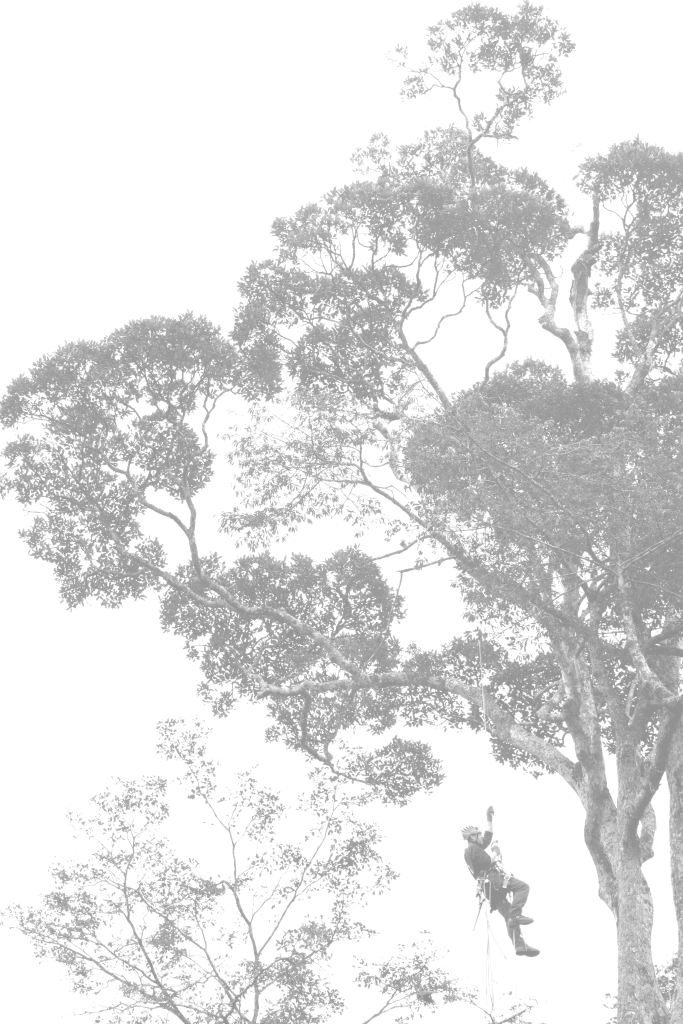
\includegraphics[width=10cm]{Filigrane}
	 \end{textblock}
	\begin{textblock}{140}[0, 1](50, 262)
		\normalfont	Version: \thedate
	\end{textblock}
	\newpage
	~\\ % Print a character or the page will not exist
	\begin{textblock}{140}(40, 40)
		#1
	\end{textblock}
	\begin{textblock}{140}[0,1](40, 270)
		\centering
    \includegraphics[width=5cm]{Logo-Lab}\\ \bigskip
		UMR \'Ecologie des forêts de Guyane\\
		\url{http://www.ecofog.gf}\\[3\baselineskip]
		Les opinions émises par les auteurs sont personnelles et n’engagent ni l’UMR EcoFoG ni ses tutelles.

    \tiny{Photographie en couverture: Hadrien Lalagüe}
	\end{textblock}
	\newpage
}

% PhD / HDR Thesis
%%%%%%%%%%%%%%%%%%%%%%%%%%%%%%%%%%%%%%%%%%%%%%%%%%%%%%%%%%

\usepackage[DocType=PhD, ED=UG, Ets=UG, DIS=ST]{latex/pdgUniv}

\specialty{Écologie}
\defencedate{1er janvier 2018}
\lab{Écologie des Forêts de Guyane}
% ==================
% Setup people like your boss, the jury team and the referees
% - First you need to define how number they will be in each category
%   It is done with the commands \nboss{n}, \nreferee{n} and \njudge{n}.
%   You can define more people in each category than the number given
%   but only the first "\npeople" will be print.
% - Then use the command \makesomeone{<category>}{<number>}{<name>}{<status>}{<other>}
%   where:
%     <category> should be select in ['boss', 'referee', 'judge']
%     <number>   is the rank for printing the person.
%                Only number <= "\npeople" will be printed
%     <name>     First name and las name of the people
%     <status>   Is (s)he a "charg\'e de recher" ou un "professeur d'universit\'e"...
%     <other>    What ever string you want to add (laboratory, jury member place...).
\njudge{7}
\makesomeone{judge}{1}{Prénom NomJury1}{Professeur d'Université}{Membre du Jury}
\makesomeone{judge}{2}{Prénom NomJury2}{Professeur d'Université}{Membre du Jury}
\makesomeone{judge}{3}{Prénom NomJury3}{Professeur d'Université}{Membre du Jury}
\makesomeone{judge}{4}{Prénom NomJury4}{Professeur d'Université}{Membre du Jury}
\makesomeone{judge}{5}{Prénom NomJury5}{Professeur d'Université}{Membre du Jury}
\makesomeone{judge}{6}{Prénom NomJury6}{Professeur d'Université}{Membre du Jury}
\makesomeone{judge}{7}{Prénom NomJury7}{Professeur d'Université}{Membre du Jury}



% End of preamble
%%%%%%%%%%%%%%%%%%%%%%%%%%%%%%%%%%%%%%%%%%%%%%%%%%%%%%%%%%


\begin{document}
\frontmatter

% Title page
%%%%%%%%%%%%%%%%%%%%%%%%%%%%%%%%%%%%%%%%%%%%%%%%%%%%%%%%%%


\makeflyleaf




% Before Body
%%%%%%%%%%%%%%%%%%%%%%%%%%%%%%%%%%%%%%%%%%%%%%%%%%%%%%%%%%




% Contents
%%%%%%%%%%%%%%%%%%%%%%%%%%%%%%%%%%%%%%%%%%%%%%%%%%%%%%%%%%

\LargeMargins
{
\hypersetup{linkcolor=}
\setcounter{tocdepth}{3}
\tableofcontents
}


% Body
%%%%%%%%%%%%%%%%%%%%%%%%%%%%%%%%%%%%%%%%%%%%%%%%%%%%%%%%%%

\LargeMargins
\begin{verbatim}
## Warning: package 'bookdown' was built under R version 3.3.3
\end{verbatim}

\begin{verbatim}
## Warning: package 'knitr' was built under R version 3.3.3
\end{verbatim}

\begin{verbatim}
## Warning: package 'rmarkdown' was built under R version 3.3.3
\end{verbatim}

\begin{verbatim}
## Warning: package 'kableExtra' was built under R version 3.3.3
\end{verbatim}

\mainmatter

\chapter{Introduction générale}\label{introduction-generale}

\section{Les forêts tropicales humides, au coeur de l'avenir
planétaire}\label{les-forets-tropicales-humides-au-coeur-de-lavenir-planetaire}

\subsection{Les écosystèmes forestiers, aujourd'hui
incontournables}\label{les-ecosystemes-forestiers-aujourdhui-incontournables}

Les forêts représentent 30\% de la surface du globe et sont attachée à
des valeurs historique, culturelle et patrimoniale fortes et ont leur
place au coeur des programmes politiques, de recherche et de
développement. Elles maintiennent notre environnement naturel, du
climat, de la diversité biologique et de la qualité de l'eau, de l'air
et des sols. Elles assurent aussi le bien être des populations, la
sécurité alimentaire et le développement de nos sociétés en tant que
sources de revenus et d'opportunités de développement ``vert''
\autocites{FRA2015}{Tilman2014}.

Par ``forêt'' ou ``ecosystème forestier'' on entend une unité
fonctionnelle dont les arbre sont les composants essentiels définie par
les assemblages de plantes, animaux et microorganismes et leur
environnement définissant \autocite{FRA2000}. Ces écosystèmes
accueillent la diversité animale et végétale et les taux d'endémismes
les plus importants du globe et correspondent aux régions restées les
moins anthropisées à forts enjeux de conservation
\autocites{Myers2000}{Mittermeier2003}. Les forêts entretiennent les
cycles de l'eau et des nutriments (azote, phosphore, etc), recyclés par
leurs réseau racinaire, et régulent la fertilité des sols, les
températures, et les précipitations locales
\autocites{Malhi2008}{Isbell2017}. Ce sont également des puits de
carbone de 1.1 ± 0.8 PgC.yr\textsuperscript{--1} et sont donc un élément
central de la régulation des émissions gaz à effet de serre (\emph{GES})
et des changements globaux. Elles permettent en effet d'une part de
compenser les émissions de GES dans l'atmosphère, mais peuvent d'autre
part devenir une importante source de carbone lorsque le carbone stocké
dans leur biomasse est libéré par la dégradation de l'écosystème
\autocites{Pan2011}{Roy2017}.

Enfin, les forêts interconnectées depuis toujours aux populations
humaines représentent des dimensions culturelles, spirituelles et
patrimoniales importantes. A l'échelle globale la subsistance de 500
millions de personnes dépend directement des forêts qui sont une source
de biens allant de la nourriture (via la chasse et la collecte de
produits forestiers non ligneux comestibles), à l'eau, aux matériaux de
construction, et à l'énergie (vie l'utilisation du bois pour le
chauffage et la cuisson des aliments). L'exploitation forestière quant à
elle représentait \textasciitilde{} 1\% du PIB mondial et une part
importante de l'emploi en 2011 et la dendroénergie reste l'une des
principales sources d'énergie \autocites{CBDdiversity2011}{FAO2014}.

\subsection{Des écosystèmes menacés, en particulier sous les
tropiques}\label{des-ecosystemes-menaces-en-particulier-sous-les-tropiques}

Malgré leur caractère irremplaçable et les multiples biens et services
qu'ils rendent, les écosystèmes forestiers subissent une dégradation
croissante, ayant abouti à une perte de 3\% de leur surface globale
entre 2013 et 2015 \autocite{FAO2009}. Les forêts sont en effet soumises
à de fortes pressions anthropiques, telles que changements d'usage des
terres, introduction d'espèces invasives et exploitation du bois et de
la chasse; et aux changements globaux qui provoquent des modifications
climatiques et atmosphériques et augmentent la fréquence des événements
extrêmes (sécheresses, incendies, inondations\ldots{})
\autocite{Pachauri2014}. Une prise de conscience globale, entérinée par
la conférence des nations unies sur l'environnement et le développement
à Rio en 1992, a motivé de nombreuses politiques de surveillance , de
conservation de la biodiversité et de préservation du fonctionnement des
forêts. Malgré tout, les pressions exercées sur les forêts restent
croissantes et mettent en jeu les biens et services qu'elles rendent
\autocites{Summit1992}{Schlaepfer2000}{Dirzo2003a}{Morales-Hidalgo2015}.

Ce contexte concerne en particulier les forêts tropicales, où les
menaces anthropiques pèsent d'autant plus gravement que leur rôle est
déterminant au niveau mondial \autocites{Dirzo2003a}{Hansen2013}. Les
bassins forestiers tropicaux, qui représentent 1.3 million d'hectares,
accueillent la diversité biologique la plus élevée au monde. Ils
correspondent également aux plus grandes surfaces de forêts anciennes
``primaires'', qui n'ont pas connu de forte perturbation anthropique
\autocites{Gentry1988}{FAO2011}. Ces régions de forêt tropicale,
historiquement peu peuplées, connaissent aujourd'hui une croissance
démographique moyenne de près de 1,4\% par an entraînant des pressions
croissantes de chasse, d'exploitation du bois, de conversion en terres
agricoles et de dégradation en forêts secondaires \autocite{Asner2009}.

Dans la logique de préservation des écosystèmes forestiers, une
attention particulière doit ainsi être portée aux zones tropicales et
aller vers une meilleure compréhension de leurs dynamiques et de leur
fonctionnement.

\subsection{La biodiversité: clé du fonctionnement des forêts
tropicales}\label{la-biodiversite-cle-du-fonctionnement-des-forets-tropicales}

Le fonctionnement des écosystèmes forestiers repose largement sur leur
biodiversité, \emph{i.e} la diversité biologique des plantes, animaux,
champignons et microorganismes qui les constituent, de leur variabilité
génétique et phénotypique, et de la variabilité de leur assemblage en
commmunautés. Les pressions exercées sur les forêts n'épargnent pas leur
diversité d'écosystèmes, de gènes et d'espèces dont une part
significative a déjà été anéantie et continue de disparaitre
irréversiblement. Cette érosion de la biodiversité est déjà qualifiée de
sixième extinction de l'ère moderne
\autocites{Vitousek1997}{Cardinale2012}.

Dans ce contexte, la littérature s'est largement intéressée au rôle de
la biodiversité et à son érosion, dont l'impact sur le fonctionnement,
les biens et les services des écosystèmes est déjà prouvé
\autocites{Sterner2002}{Cardinale2012}{Tilman2014}. La disparition
d'espèces en elle-même, d'une part, représente une dégradation du
patrimoine naturel mondial. D'autre part, selon l'originalité biologique
des espèces et l'existence d'autres espèces biologiquement proches leur
disparition peut signifier la perte de leur rôle dans l'écosystème et
avoir des conséquences importantes et inattendues, comme ce peut être le
cas pour des espèces \emph{clé de voûte}
\autocites{Jones1994}{Power1996}{Gardner2007}. Par ailleurs, la
diversité biologique implique une complémentarité entre individus
permettant d'optimiser l'utilisation et la transformation des resources
naturelles. Elle détermine donc la productivité des écosystèmes et les
flux de nutriments, d'eau et de carbone à la base des processus
écosystémiques. Ces processus entre l'environnement et les organismes,
comme les chaînes trophiques, les migrations ou le stockage stockage,
dépendent des stratégies spécifiques d'utilisation des ressources et
donc de la composition et de la diversité en espèces des communautés
\autocite{Begon2006}. Enfin, la diversité des communautés détermine la
stabilité des écosystèmes. Une diversité importante limite d'une part
l'impact des maladies, des espèces invasives, des variations
environnementales, etc et augmente la résistance des écosystèmes et
facilite d'autre part la restauration de l'état avant perturbation et
augmente la résilience de l'écosystème\autocite{Elmqvist2003}.

Le rôle de la biodiversité et l'impact de son érosion ont déjà été
prouvé, mais l'impact des perturbations actuelles sur les trajectoires
de composition et de diversité des écosystèmes demeurent parfois
imprécis. Il est nécessaire de mieux expliciter la réponse des
communautés en termes de composition et de diversité pour en anticiper
l'impact sur le fonctionnement et l'évenir des forêts.

\section{Comment mesurer la diversité biologique
?}\label{comment-mesurer-la-diversite-biologique}

La notion de biodiversité correspond à la diversité des espèces
vivantes, de leurs gènes et de leur phénotype, des interactions
écologiques qu'elles ont entre elles et avec leur environnement, et de
leurs assemblages en communautés \autocite{Loreau2005}. La biodiversité
est donc la somme de la variabilité biologique, des gènes jusquà
l'assemblages de sespèces en écosystèmes. Mesurer la biodiversité permet
donc d'appréhender les mécanismes écologiques fondamentaux qui régissent
les écosystèmes et leurs dynamiques spatiales et temporelles
\autocites{Purvis2000}{Loreau2005}.

\subsection{Assemblage et structure des
communautés}\label{AbundanceDistribution}

Nous nous intéressons ici aux écosystèms forestiers dont les arbres sont
les éléments essentiels et dont la diversité reflète celles des autres
groupes \autocite{Guitet2017}. Notre étude de la la diversité des forêts
reviendra ici à mesurer leur diversité en essences forestières. Une
communauté, qu'elle soit végétale, animale ou microbienne, est
constituée d'espèces dont les effectifs sont différents: certaines
seront très abondantes, d'autres moyennement communes et d'autres
encore, souvent la majorité, rares. La façon la plus simple et immédiate
de décrire une communauté est de donner la distribution d'abondance de
ses espèces, qui représente les proportions d'espèces abondantes rapport
aux espèces communes ou rares. Cette distribution bien que variable
d'une communauté à l'autre, est régie par des lois écologiques lui
donnant invariablement une courbe en creux \ref{fig:AbdDist}
\autocite{McGill2007}.

\begin{Shaded}
\begin{Highlighting}[]
\NormalTok{knitr}\OperatorTok{::}\KeywordTok{include_graphics}\NormalTok{(}\StringTok{"ExternalFig/SpeciesAbdDist.jpg"}\NormalTok{)}
\end{Highlighting}
\end{Shaded}

\begin{SCfigure}

{\centering 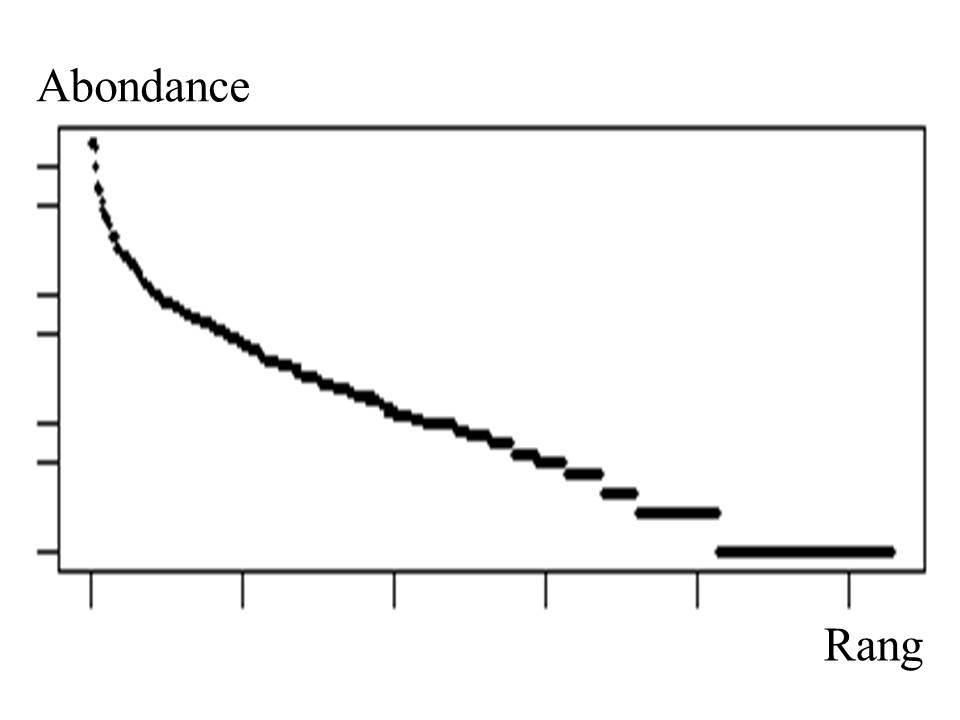
\includegraphics[width=0.6\linewidth]{ExternalFig/SpeciesAbdDist} 

}

\caption{Exemple de distribution d'abondance pour une communauté d'arbres en forêt tropicale humide}\label{fig:AbdDist}
\end{SCfigure}

Cette uniformité des distributions d'abondance a motivé le développement
de modèles proposant des relations mathématiques entre le nombre
d'espèces et leur abondance. Ces modèles reflètent le lien entre
l'importance d'une espèce et la quantité de resources qu'elle mobilise
dans l'environnement pour son développement: plus une espèce sera
comptétitive, plus elle sera abondante. Ce lien s'établit vis à vis de
la ressource la plus limitante: il peut s'agir de la lumière atteignant
le sol en forêt tropicale, de l'eau dans les milieux arides, de
l'espace, etc \autocites{findref}[ dans
Asner2004spatial-and-temporal]{Johns1996}. Prédire une distribution
d'abondance revient à prédire la répartition de la ressource limitante
entre les espèces de la communauté. De nombreux modèles prédictifs ont
été proposés, des modèles statistiques divisant aléatoirement la
ressource selon une loi de propabilité qui détermine les effectifs de
chaque espèce, ou des modèles mécanistes divisant la resource selon une
formule prédéterminée, par exemple en la divisant successivement selon
une fraction constante
\autocites{Fisher1943}{Motomura1932}{Tokeshi1993}{Magurran1988}.

Ces modèles, éprouvés pour de nombreuses communautés, ont montré une
bonne représentation des communautés réelles et révèlent ainsi les
règles écologiques qui en régissent l'assemblage. Ce sont donc des
outils adéquats pour comparer les communautés et d'en interpréter les
différences. Manipuler une distribution d'abondance n'est cependant pas
le plus aisé et ne permet pas de quantifier les différences entre
communautés. A partir de ces distribution et des modèle proposés pour
les représeter, en revanche, de nombreuses mesures permettent de
quantifier le nombre d'espèces, la forme des distribution, ou encore
l'homogénéité des abondances sépcifiques. Ces indicateurs sont les
indices de diversité, résumant de façon quantifiable les
caractéristiques des distributions d'abondance.

\subsection{Les composantes de la
diversité}\label{les-composantes-de-la-diversite}

La biodiversité d'une communauté est souvent assimilée à sa richesse en
espèces. L'abondance des différentes espèces est cepedant essentiel pour
décrire une communauté \ref{ref:AbundanceDistribution}. Une espèce
dominante n'apportera pas la même contribution à l'écosystème qu'une
espèce rare: une communauté dominée par une ou deux espèces très
abondantes sera intuitivement moins diverse qu'une autre avec autant
d'espèces mais aux abondances équivalentes. En plus de refléter les
règles fondamentales d'assemblage des communautés, l'équitabilité d'une
communauté peut être bien plus révélatrice du fonctionnement des
écosystèmes que leur richesse ou leur composition. Cette idée est
illustrée par l'hypothèse du ratio de biomasse selon laquelle les
espèces dominantes caractérisent bien plus les écosystèmes que les
espèces rares. Les espèces peu communes n'ont en effet qu'une influence
à long terme en tant que potentielles futures espèces dominantes s'il
s'opère un changement de l'environnement, ou pas d'influence si elles ne
sont que transitoires et ne persistent pas dans l'écosystème
\autocite{Grime1998}.

La richesse, simplement le nombre d'espèces recensées, et
l'équitabilité, la régularité de distribution d'abondance des espèces,
sont donc les deux composantes à prendre en compte pour mesurer la
diversité d'une communauté \ref{fig:RichEqu}
\autocites{Whittaker1965}{Magurran2004}.

\begin{Shaded}
\begin{Highlighting}[]
\NormalTok{knitr}\OperatorTok{::}\KeywordTok{include_graphics}\NormalTok{(}\StringTok{"ExternalFig/Fig_RichnessEquitability.jpg"}\NormalTok{)}
\end{Highlighting}
\end{Shaded}

\begin{SCfigure}

{\centering 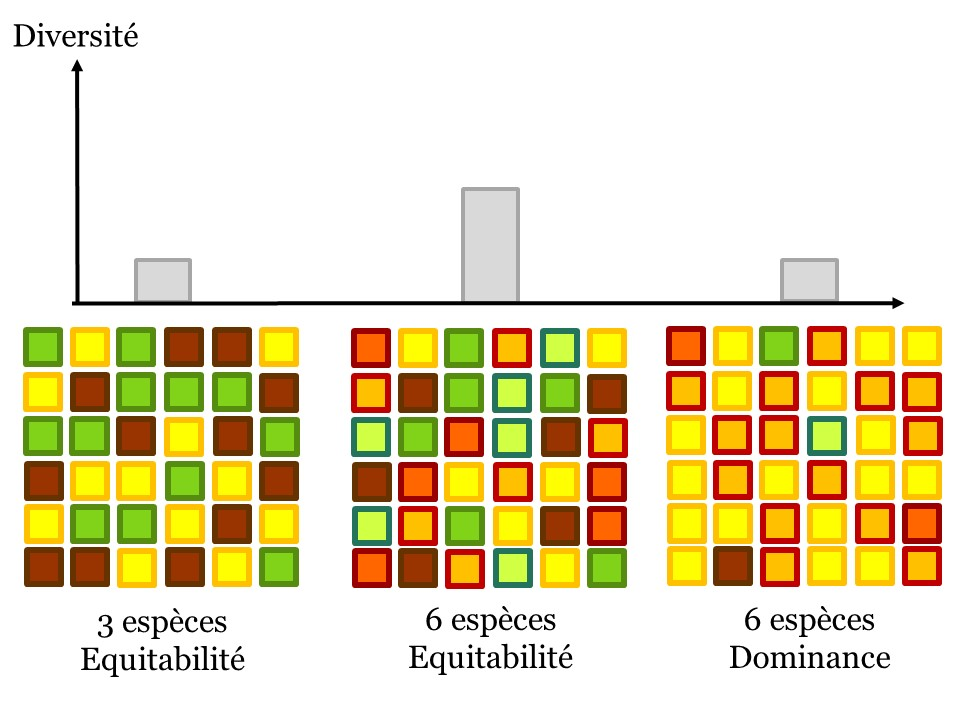
\includegraphics[width=0.6\linewidth]{ExternalFig/Fig_RichnessEquitability} 

}

\caption{Les deux composantes de la diversité taxonomique: richesse (nombre d'espèces) et équitabilité (homogeneité de répartition)}\label{fig:RichEqu}
\end{SCfigure}

Aucune mesure unique ne mesure pleinement la diversité, mais plutôt un
panel d'indices combinant différemment les composantes de la diversité.
Des familles d'indices ont été développées et regroupent les indices
mesurés selon une même formule modulable selon le poids accordé aux
différentes composantes de la diversité. La famille des indices de
diversité de Réyni, judicieuse pour l'étude des communautés végétales,
rassemble les indices mesurés selon l'équation \eqref{eq:formHCDT} modulée
par un paramètre \emph{q} appelé ``ordre de diversité'' correspond au
poids des espèces rares par rapport aux espèces abondantes
\autocite{Mendes2008}. Plus l'ordre de diversité est élevé, plus les
espèces rares sont négligées par rapport aux espèces abondantes.

\begin{equation}
^{q}H=\frac{1}{q-1}\Bigg(1-\displaystyle\sum_{s=1}^{S}p^q_s\Bigg) }
\label{eq:formHCDT}
\end{equation}

Dans cette famille d'indices de diversité se retrouvent les indices les
plus utilisés: l'ordre 0 où chaque espèce contribue de la même façon
correspond à la richesse spécifique, l'ordre 1 où richesse et
équitabilité sont également pris en compte correspond à l'indice de
Shannon, et l'ordre 2 pour lequel les espèces rares sont presque
négligées correspond à l'indice de Simpson (parfois appelé ``diversité
en espèces abondantes'')
\autocites{Shannon1948}{Simpson1949}{Patil1982}{Tothmeresz1995}.

Ces indices, s'ils sont corrects et représentatifs des différentes
composantes de la diversité, ne correspondent pas directement à un
nombre intelligible et ne permettent pas de comparer facilement des
communautés de tailles différentes. On se rapporte donc à un
\emph{nombre équivalent d'espèces} correspondant au nombre d'espèces
qu'aurait la communauté étudiée si toutes les abondances étaient égales.
Ce nombre équivalent d'espèces, ou \emph{nombre de Hill}, est obtenu par
transformation des valeurs obtenues par une exponentielle à base q
\autocite{Hill1973}.

Les mesures de diversité choisies sont donc la traduction intelligible
en nombre équivalent d'espèces d'une déclinaison d'indices combinant
richesse et équitabilité de différentes façons et qui capte toute la
structure de diversité.

\subsection{Résolution du biais
d'échantillonnage}\label{resolution-du-biais-dechantillonnage}

En pratique aucun inventaire n'est exhaustif, et l'étude de la diversité
se heurte aux biais d'échantillonnage qui sous-estiment la richesse et
faussent l'abondance des espèces. La correction de ce biais nécessite
l'estimation des abondances réelles à partir des observations et des
relations mathématiques qu'il existe entre les abondances des
différentes espèces. La première application de cette méthode correspond
à l'adaptation de la formule des fréquences de Turing
\autocite{Good1953} où l'abondance réelle *\alpha\_v* d'une espèce
observée \emph{v} fois dans un échantillonnage de \emph{n} individus est
reliée au rapport entre le nombre d'autres espèces observées également
\emph{v} fois et de celles observées \emph{v+1} fois
@ref\{eq=formGoodTuring\}:

\begin{equation}
\alpha_v=\frac{\big(v+1\big)}{n}\fraq{s^n_{v+1}}{s^n_v}
\label{eq:formGoodTuring}
\end{equation}

Les singletons (espèces observées une seule fois) et les doubletons
(espèces observées deux fois) sont particulièrement intéressants car il
permettent d'estimer le nombre \emph{s\^{}n\_0} d'espèces manquées
(observées zéro fois) et donc de corriger le biais d'échantillonnage de
la richesse, sachant que \(s^n_0=\frac{s^n_1}{n}\).

Cette relation de base a été précisée selon de nombreuses méthodes, en y
intégrant notamment la notion de \emph{taux de couverture} qui quantifie
l'effort d'échantillonnage d'un inventaire réel et permet de savoir
quelle proportion de la communauté a pu être échantillonnée
\autocite{Dauby2012}. Pour chaque inventaire, des méthodes permettant de
choisir la correction la plus adéquate ont de plus été développés et
éprouvés \autocites{Chao2015}{Marcon2015b}.

\subsection{Diversité fonctionnelle}\label{diversite-fonctionnelle}

Les mesures de diversité décrites précédemment considèrent toutes les
espèces de la même façon: la richesse compte le nombre d'espèces
distinctes, que celles-ci aient ou non les mêmes caractéristiques
fonctionnelles ou phylogénétiques. Ces mesures de diversité, dites
neutres car elles ne tiennent pas compte des caractéristiques de chaque
espèce, peuvent être étendues pour intégrer la similarité entre espèces
au sein d'une communauté. Plus les espèces d'une communauté sont
différentes plus la diversité sera élevée: dans le cas des communautés
végétales la similarité entre espèces peut être phylogénétique, en
considérant leur distance au sein d'un arbre phylogénétique, ou
fontionnelle, en considérant leurs différences morphologiques ou
physiologiques \ref{fig:RichEquSim}.

\begin{Shaded}
\begin{Highlighting}[]
\NormalTok{knitr}\OperatorTok{::}\KeywordTok{include_graphics}\NormalTok{(}\StringTok{"ExternalFig/Fig_RichnessEquitabilitySimilarity.jpg"}\NormalTok{)}
\end{Highlighting}
\end{Shaded}

\begin{SCfigure}

{\centering 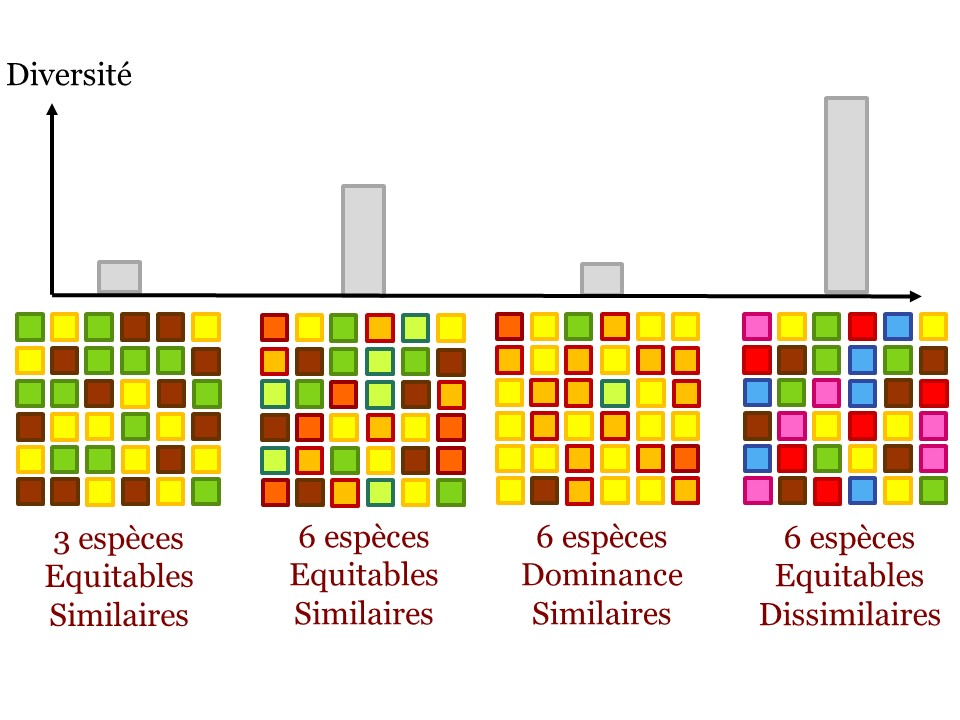
\includegraphics[width=0.6\linewidth]{ExternalFig/Fig_RichnessEquitabilitySimilarity} 

}

\caption{Troisième composante de la diversité: la similarité entre espèces basée sur des distances phylogénétiques ou taxonomiques}\label{fig:RichEquSim}
\end{SCfigure}

Ces similarités sont ensuite intégrées aux indices de diversité, au même
titre que les composantes de richesse et d'équitabilité, sous la forme
d'une matrice de distances entre espèces calculée sur la base de leur
phylogénie ou de leurs traits fonctionnels.

Les traits fonctionnels sont les caractéristiques morphologiques,
physiologiques et phénologiques des espèces, ils déterminent le
fonctionnement des individus, leur performance de croissance et de
survie, et leurs interaction avec l'environnement
\autocite{Violle2007b}. L'approche fonctionnelle décrivant les espèces
et les individus selon leurs caractéristiques biologiques plutôt que par
leur nom botanique a été largement adoptée en écologie pour appréhender
le fonctionnement et les dynamiques des communautés. Elle réduit la
dimensionnalité des communautés, nécessaire dans le cas d'écosystèmes
aussi riches que les forêt tropicales, et permet de comparer les
communautés quelle que soit leur composition en espèces
\autocites{Begon2006}{Scheiter2013}{Mouillot2013a}{Sakschewski2016}. La
trajectoire de diversité fonctionnelle d'une communauté après
perturbation est interprétable en terme d'utilisation des ressources et
de flux de matière et d'énergie, et permet d'appréhender l'impact de la
perturbation sur le fonctionnement de l'écosystème. L'approche
fonctionnelle permet enfin d'identifier les processus d'assemblage des
communautés en comparant la diversité observée à celle d'une assemblage
aléatoire. Le filtrage environnemental sera traduit par une aggrégation
des traits et une diversité fonctionnelle faible, traduisant le
sélection de certains types fonctionnels, ou au contraire une limitation
de similarité et une diversité fonctionnelle élevée,due à l'exclusion
compétitive entre espèces \autocite{Refelodie}.

L'approche fonctionnelle nécessite de choisir judicieusement les traits
intégrés aux indices de diversité. Une vaste littérature a permis
d'identifier les traits clés représentatifs de l'écologie et de la
croissance des espèces et de leur influence sur le fonctionnement de
l'écosystème \autocite{Reich2014}. Les traits foliaires tout d'abord,
représentatifs de la stratégie d'acquisition et d'allocation des
resources, ont permis de définir un ``spectre économique foliaire''
opposant les espèces à larges feuilles fines ayant une forte capacité
photosynthétique correspondant à une acquisition rapide des resources,
aux espèces à petites feuilles coriaces et résistantes. Ces stratégies
d'acquisition des resources déterminent la stratégie de croissance des
espèces: les espèces ``acquisitives'' auront une croissance rapide et
une courte durée de vie tandis que les espèces ``conservatives'' auront
une croissance plus lente mais une meilleure résistance aux conditions
environnementales éprouvantes \autocites{Reich1997}{Wright2004}. Un
gradient similaire s'applique aux traits racinaires et aux propriétés du
bois, opposant les espèces aux tissus légers à courte durée de vie
permettant une croissance rapide à celles aux tissus denses plus
résistants et mobilisant plus de ressources
\autocites{Chave2009}{Valverde-Barrantes2017}. Ces traits fonctionnels
mesurables à l'échelle de l'individus déterminent sa stratégie
écologique et sa performance et sont associés à des \emph{traits
d'histoire de vie} mesurables à l'échelle de l'espèce. Parmi ces traits
d'histoire de vie la masse des graines et la hauteur moyenne maximale
des arbres à l'âge adulte ont montré être particulièrement
représentatifs des stratégies de croissance, de survie et de
reproduction \autocites{Westoby1998}{Herault2011}.

La combinaison de l'ensemble de ces traits spécifique, foliaires,
racinaires et du bois permet d'appréhender précisément la stratégie
fonctionnelle des espèces, leurs préférences écologiques et leur
performance de croissance et de survie. L'engouement récent de
l'écologie pour l'approche fonctionnelle a de plus permis la création de
bases de données fonctionnelles conséquentes et standardisées qui
rendent possibles l'approche fonctionnelle à l'échelle des communautés
{[}\textcite{Kattge2011}; \textcite{Perez-Harguindeguy2013};
{[}\^{}1{]}{]}

{[}\^{}1{]} \url{http://www.ecofog.gf/Bridge/}

\section{La Guyane Française et l'exemple de la station de
Paracou}\label{la-guyane-francaise-et-lexemple-de-la-station-de-paracou}

Le bassin Amazonien est la plus riche des trois principales régions de
forêt tropicale humide \autocite{Gentry1988}. La Guyane française en est
une région française de 83 846 km\^{}2, au Nord-Est du continent
sud-américain entre le Surinam et le Brésil, recouverte à 95\% par la
forêt tropicale humide.

\subsection{Le contexte Guyanais}\label{le-contexte-guyanais}

La région appartient au bouclier des Guyanes qui s'étend de l'Amapa au
Brésil jusqu'au delta de l'Orénoque au Venezuela. Formé il y a plus de 2
milliards d'années, le bouclier des Guyanes correspond aujourd'hui à un
assemblage d'unités géomorphologiques façonnées par une succession
d'épisodes géologiques, climatiques et marins. Ces unités intègrent des
conditions pédologiques, climatiques et topographiques déterminant la
composition et la diversité du couvert végétal et les processus
écologiques qui les régissent, tels que les migrations et le filtrage
environnemental \autocite{Guitet2015}.

Le relief Guyanais est une alternance de collines, jusqu'à 50m
d'altitude, et de bas-fonds humides qui correspond à une forte
variabilité de la pente et du sol. La profondeur et la composition des
sols et leur capacité de rétention et de drainage de l'eau sont ainsi
très hétérogène \autocites{Ferry2010}{Robert2003}. Les sols sont des
Acrisols recouvrant une couche de saprolite transformée peu perméable
qui entraîne un drainage latéral des précipitations.

Le climat est un climat tropical humide, davantage marqué par le régime
des précipitations que par celui des températures. La température
moyenne est 26°C et reste constante au cours de l'année tandis les
précipitations moyennes annuelles varient de 2 000 à 4 000
mm.an\textsuperscript{-1} et montrent une grande variabilité spatiale et
temporelle. Les précitations suivent un gradient décroissant marqué
d'est en ouest et une forte variabilité au cours de l'année, avec une
saison humide entre novembre et avril et une saison sèche d'avril à
mi-juillet durant laquelle les précipitations sont inférieures à 50 mm
\autocite{Wagner2011}.

La forêt Guyanaise est une forêt équatoriale sempervirente ombrophile de
plaine. D'une richesse incroyable, elle accueille plus de 7 000 espèces
végétales (hors champignons) dont 1 500 espèces d'arbres et une richesse
faunistique toute aussi incroyable \autocite{DeNoter2008}. La
composition spécifique des arbres connait également une importante
variabilité spatiale. Plusieurs patrons de composition on été mis en
évidence selon un gradient du nord-ouest, où dominent les familles
botaniques des \emph{Lecythidaceae} et \emph{Cesalpinaceae}, au sud-est,
où dominent \emph{Burseraceae} et \emph{Mimosaceae}. Ces patrons ont
montré être déterminés en particulier par une combinaison de la
topographie et de la pédologie \autocites{Sabatier1989}[ cf
Toto]{Sabatier1997}{Guitet2015}.

\subsection{Paracou, plus de 30 de suivi de la forêt
Amazonienne}\label{paracou-plus-de-30-de-suivi-de-la-foret-amazonienne}

Le dispositif de Paracou, installé entre les communes de Kourou et
Sinnamary (5°18'N and 52°53'W), a été mis en place en 1984 pour étudier
l'impact de l'exploitation forestière sélective sur les peuplements. Le
dispositif correspond à l'origine à 12 parcelles de 6.25 ha ayant subi
en 1984 un gradient de trois intensités d'abattage, d'éclairices et de
coupe de bois de chauffage. Le traitement de perturbation a été attribué
selon un dispositif aléatoire de trois réplications de 4 traitements:
parcelles témoins sans intervention (\emph{T0}), traitement 1 avec
coupes d'abattage (\emph{T1}), traitement 2 avec abattage et éclaircies
par \textbf{poison girdling} (\emph{T2}), traitement 3 avec abattage,
éclaircies et coupe de bois de chauffage (\emph{T3})
\ref{tab:InterventionTable}.

\begin{Shaded}
\begin{Highlighting}[]
\NormalTok{textExp<-}\StringTok{ }\KeywordTok{do.call}\NormalTok{(rbind,}\KeywordTok{list}\NormalTok{(}\KeywordTok{c}\NormalTok{(}\StringTok{"DBH $}\CharTok{\textbackslash{}\textbackslash{}}\StringTok{geq$ 50 cm, espèces commerciales, ~ 10 arbres/ha"}\NormalTok{,}\StringTok{" "}\NormalTok{,}\StringTok{""}\NormalTok{,}\StringTok{"[12}\CharTok{\textbackslash{}\textbackslash{}}\StringTok{%-33}\CharTok{\textbackslash{}\textbackslash{}}\StringTok{%]"}\NormalTok{),}
         \KeywordTok{c}\NormalTok{(}\StringTok{"DBH $}\CharTok{\textbackslash{}\textbackslash{}}\StringTok{geq$ 50 cm, espèces commerciales, ~ 10 arbres/ha"}\NormalTok{,}\StringTok{"DBH $}\CharTok{\textbackslash{}\textbackslash{}}\StringTok{geq$40 cm, espèces non-commerciales,~ 30 arbres/ha"}\NormalTok{,}\StringTok{" "}\NormalTok{,}\StringTok{"[33}\CharTok{\textbackslash{}\textbackslash{}}\StringTok{%-56}\CharTok{\textbackslash{}\textbackslash{}}\StringTok{%]"}\NormalTok{),}
         \KeywordTok{c}\NormalTok{(}\StringTok{"DBH $}\CharTok{\textbackslash{}\textbackslash{}}\StringTok{geq$50 cm, espèces commerciales, ~ 10 arbres/ha"}\NormalTok{,}\StringTok{"DBH $}\CharTok{\textbackslash{}\textbackslash{}}\StringTok{geq$50 cm, espèces non-commerciales,~ 15 arbres/ha"}\NormalTok{,}\StringTok{"40 cm $}\CharTok{\textbackslash{}\textbackslash{}}\StringTok{leq$ DBH $}\CharTok{\textbackslash{}\textbackslash{}}\StringTok{leq$ 50 cm, espèces non-commerciales,~ 15 arbres/ha"}\NormalTok{,}\StringTok{"[35}\CharTok{\textbackslash{}\textbackslash{}}\StringTok{%-56}\CharTok{\textbackslash{}\textbackslash{}}\StringTok{%]"}\NormalTok{)))}
\KeywordTok{colnames}\NormalTok{(textExp)<-}\KeywordTok{c}\NormalTok{(}\StringTok{"Abattage"}\NormalTok{, }\StringTok{"Eclairices"}\NormalTok{, }\StringTok{"Bois de chauffage"}\NormalTok{, }\StringTok{"}\CharTok{\textbackslash{}\textbackslash{}}\StringTok{% Biomasse aérienne perdue"}\NormalTok{)}
\KeywordTok{rownames}\NormalTok{(textExp)<-}\KeywordTok{c}\NormalTok{(}\StringTok{"T1"}\NormalTok{,}\StringTok{"T2"}\NormalTok{,}\StringTok{"T3"}\NormalTok{)}

\NormalTok{knitr}\OperatorTok{::}\KeywordTok{kable}\NormalTok{(textExp, }\DataTypeTok{caption=}\StringTok{"Intensité des traitements appliqués aux parcelles perturbées de Paracou."}\NormalTok{, }\DataTypeTok{booktabs =} \OtherTok{TRUE}\NormalTok{)}
\end{Highlighting}
\end{Shaded}

\begin{table}

\caption{\label{tab:InterventionTable}Intensité des traitements appliqués aux parcelles perturbées de Paracou.}
\centering
\begin{tabular}[t]{lllll}
\toprule
  & Abattage & Eclairices & Bois de chauffage & \textbackslash{}\% Biomasse aérienne perdue\\
\midrule
T1 & DBH \$\textbackslash{}geq\$ 50 cm, espèces commerciales, \textasciitilde{} 10 arbres/ha &  &  & [12\textbackslash{}\%-33\textbackslash{}\%]\\
T2 & DBH \$\textbackslash{}geq\$ 50 cm, espèces commerciales, \textasciitilde{} 10 arbres/ha & DBH \$\textbackslash{}geq\$40 cm, espèces non-commerciales,\textasciitilde{} 30 arbres/ha &  & [33\textbackslash{}\%-56\textbackslash{}\%]\\
T3 & DBH \$\textbackslash{}geq\$50 cm, espèces commerciales, \textasciitilde{} 10 arbres/ha & DBH \$\textbackslash{}geq\$50 cm, espèces non-commerciales,\textasciitilde{} 15 arbres/ha & 40 cm \$\textbackslash{}leq\$ DBH \$\textbackslash{}leq\$ 50 cm, espèces non-commerciales,\textasciitilde{} 15 arbres/ha & [35\textbackslash{}\%-56\textbackslash{}\%]\\
\bottomrule
\end{tabular}
\end{table}

En 1990, trois parcelles de 6.25ha et une parcelle de 25ha (parcelles
13, 14, 15 et 16) ont été ajoutées au dispositif pour l'étude et le
suivi de la diversité en forêt non perturbée \ref{fig:ParacouDesign}.

\begin{Shaded}
\begin{Highlighting}[]
\NormalTok{knitr}\OperatorTok{::}\KeywordTok{include_graphics}\NormalTok{(}\StringTok{"ExternalFig/Paracou.jpg"}\NormalTok{)}
\end{Highlighting}
\end{Shaded}

\begin{SCfigure}

{\centering \includegraphics[width=0.6\linewidth]{ExternalFig/Paracou} 

}

\caption{Dispositif expérimental de Paracou, schéma des 16 parcelles de suivi des dynamiques forestières. La couleur des parcelles indique l'intensité de perturbation appliquée à 9 des parcelles en 1984 (voir le tableau 1.}\label{fig:ParacouDesign}
\end{SCfigure}

Sur l'ensemble du dispositif sont recensées 591 espèces d'arbres
appartenant à 223 genre et 64 familles botaniques, principalement les
\emph{Fabaceae}, les \emph{Chrisobalanaceae}, les \emph{Lecythidaceae}
et les \emph{Sapotaceae}. Les températures annuelles atteignent 26°C et
les précipitations 2 980 mm.an\textsuperscript{-1} de mi-août à
mi-novembre, avec une saison sèche d'un mois en mars
\autocite{Wagner2011}.

\subsection{Méthodes d'inventaires}\label{methodes-dinventaires}

Depuis la mise en place du dispositif en 1984 toutes les parcelles sont
inventoriées chaque année à la saison sèche à partir de mi-juillet. Tous
les arbres de plus de 10 cm de diamètre à 1.30 m (diamètre à hauteur de
poitrine, \emph{DBH} en anglais) sont identifiés, marqués d'un numéro et
cartographiés. Les arbres morts sont relevés chaque années et notés en
précisant le type mort (mort sur pied, chablis primaire ou chablis
secondaire).

Lorsqu'un arbre atteint 10 cm il est \emph{recruté} et sera mesuré
chaque année. Il est identifié dans un premier temps par un nom
\emph{vernaculaire}, ou nom commun, attribué par l'équipe de terrain. En
1984, 62 espèces commerciales étaient identifiées par un nom commun
propre tandis que toutes les autres espèces étaient regroupées sous deux
noms vernaculaires distinguant seulement les palmiers des espèces
arborées. Cette première identification s'est précisée par la suite et
aujourd'hui 235 noms vernaculaires différents sont recensés pour
l'ensemble du dispositif sur les 30 ans de suivi. Des campagnes
d'identification botanique au cours desquelles les arbres sont
identifiés au niveau espèce ont été mises en place à partir de 2003 et
se poursuivent tous les 5 à 6 ans.

L'histoire des inventaires botaniques s'étant construite petit à petit
au gré des nouveaux projets et des forces en présence, la précision et
le taux d'identification botaniques sont variables au cours du temps et
entre les parcelles. Ceci génère des incertitudes taxonomiques
significatives notamment au regard des arbres n'ayant pu être identifiés
qu'au niveau vernaculaire, par exemple lorsque l'individu est mort avant
d'avoir pu être identifié au cours d'une campagne botanique. Les noms
vernaculaires eux-mêmes génèrent de l'incertitude taxonomique: un nom
vernaculaire correspond souvent à plusieurs noms botaniques et
inversement, un nom botanique peut correspondre à plusieurs noms
vernaculaires \autocite{Oldeman1968}.

\section{Problématique et plan de la
thèse}\label{problematique-et-plan-de-la-these}

La thèse présentée ici vise à identifier la réponse aux perturbations
d'une forêt tropicale naturelle en termes de diversité taxonomique et
fonctionnelle et à en interpréter les mécanismes sous-jacents. Le
document s'articule en trois chapitres qui prennent la forme d'articles
en cours de rédaction (pour le moment!).

\begin{itemize}
\item
  Le premier chapitre présente la méthode de propagation des
  incertitudes taxonomiques permettant de mesurer la diversité en tenant
  compte de l'hétérogéneité d'identification botanique. Nous proposons
  l'application de cette méthode dans le cas d'inventaires forestiers,
  dans la perspective de valoriser les inventaires pré-exploitations
  pour le suivi de la diversité forestière. Nous présenterons ensuite
  l'adaptation de cette méthode au cas des dispositifs expérimentaux,
  aux contraintes d'identification différente, qui sera utilisée dans la
  suite de ce travail.
\item
  Dans le deuxième chapitre seront présentées les trajectoires de
  composition et de diversité taxonomique et fonctionnelle pour les
  parcelles de Paracou. Ces trajectoires montrent la réponse unimodale
  de la composition et de la diversité taxonomique et fonctionnelle des
  peuplements après exploitation. La cinétique et le maximal de la
  divergence par rapport à l'état initial sont positivement corrélés à
  l'intensité d'exploitation. Les trajectoires de diversité valident la
  théorie des perturbations intermédiaires qui suppose une augmentation
  de la diversité après exploitation. Il existe cependant une
  décorrélation entr les trajectoires de diversité taxonomique et
  fonctionnelle suggérant une redondance fonctionelle des peuplements
  naturels qui n'est pas restaurée même 30 ans après exploitation.
\item
  Le troisième chapitre correspond à une analyse du processus de
  recrutement après exploitation. Approcher les trajectoires de
  diversité sous l'angle des processus démographiques permet de préciser
  le filtrage environnemental déterminant une population des recrutés
  significativement différente du peuplement en place, confirmant ainsi
  la théorie des perturbations intermédiaires. Cette approche permet de
  plus de délimiter trois phases de recrutement, qui mobilisent
  successivement les arbres adultes en place au moment de la
  perturbation, les semis ou les juvéniles, puis les graines de la
  banque du sol dans le cas des perturbations les plus intenses. La
  comparaison du recrutement avec le peuplement initial avant
  exploitation confirme la restauration de l'état initial mais la
  mobilisation de la banque de graines interroge sur sa résilience après
  des perturbations les plus intenses.
\end{itemize}

\chapter{Article 1 : Des inventaires forestiers aux trajectoires de
diversité: le problème universel de
l'incertitude}\label{article-1-des-inventaires-forestiers-aux-trajectoires-de-diversite-le-probleme-universel-de-lincertitude}

Malgré les enjeux liés aux forêts tropicales et l'urgence d'en préserver
l'intégrité et le fonctionnement, seule une petite fraction de leur
diversité est connue. Le nombre d'espèces inventoriées sous les
tropiques ne correspondant qu'à une observation unique
\autocite{Feeley2011} présume de l'ampleur de notre méconnaissance et
rend impossible toute supposition sur la distribution des espèces et
leurs dynamiques. Il est essentiel d'améliorer notre connaissance du
vivant, en fournissant un plus grand effort d'échantillonnage et en
valorisant toute connaissance déjà disponible.

Le coût des inventaires en temps, en main d'oeuvre et en moyens,
d'autant plus important que le niveau de l'inventaire est précis,
implique de travailler également à des méthodes pour valoriser tout type
d'inventaires \autocite{Baraloto2012}. Dans le cas de l'étude des
peuplements forestiers, les inventaires d'exploitation peu coûteux et
couvrant des surfaces larges sont une source d'information
incontournable \autocites{terSteege2000}{Guitet2014}.

\section{Noms vernaculaires et propagation des incertitudes
taxonomiques}\label{noms-vernaculaires-et-propagation-des-incertitudes-taxonomiques}

Ces inventaires ne sont cependant généralement pas réalisés en noms
scientifiques mais noms vernaculaires, qui sont mieux connus, plus
faciles à attribués car basés sur des critères morphologiques, culturels
ou d'usage et qui ne nécessitent pas de vérification botanique
ultérieure à partir d'herbiers. Cette simplicité se fait cependant au
détriment de la fiabilité des noms vernaculaires, qui correspondent à
plusieurs espèces botaniques et varient avec le temps et les équipes de
terrain \autocite{Oldeman1968}. Pour valoriser ces inventaires il est
donc nécessaire d'évaluer l'impact de l'incertitude taxonomique sur la
fiabilité et la sensibilité des mesures de diversité. Nous proposons ici
une méthode permettant de propager l'incertitude de détermination
taxonomique des noms vernaculaires aux mesures de la diversité.

Dans un premier temps nous appliquons cette méthode au contexte des
inventaires d'exploitation en noms vernaculaires pour en estimer la
fiabilité et la robustesse selon le degré d'indétermination botanique,
et proposer un protocole d'inventaire standardisé. Dans ce cas les
identifications botaniques fiables concernent quelques espèces cibles,
emblématiques ou ayant une certaine valeur commerciale ou de
conservation. Le degré d'indétermination botanique correspond alors au
nombre d'espèces identifiées systématiquement par leur nom vernaculaire
plutôt que botanique. Dans un deuxième temps nous adaptons la méthode au
contexte des dispositifs expérimentaux pour pallier l'inévitable
variabilité des pratiques d'inventaires. Dans ce cas les arbres
identifiés uniquement par un nom vernaculaire sont les individus n'ayant
pu être identifiés, que l'identification soit impossible ou qu'ils
soient mort avant le passage du taxonomiste. Le degré d'indétermination
correspond au nombre d'arbres sans identification botanique et concerne
potentiellement toutes les espèces de la communauté.

\section{Article 1 \_ Inescapable Taxonomists: Workable Biodiversity
Management Must Base on a Minimum Field
Work}\label{article-1-_-inescapable-taxonomists-workable-biodiversity-management-must-base-on-a-minimum-field-work}

\section{La recherche et les suivis à long terme: application de la
méthode de propagation aux inventaires de
Paracou}\label{la-recherche-et-les-suivis-a-long-terme-application-de-la-methode-de-propagation-aux-inventaires-de-paracou}

\subsection{Profils d'incertitude
taxonomique}\label{profils-dincertitude-taxonomique}

A la différence des inventaire sd'exploitation, dans le cas des
dispositifs expérimentaux le degré d'indétermination taxonomique
correspond à un pourcentage d'arbres, toutes espèces confondues, n'ayant
pas été identifiés au niveau spécifique. Sur le même principe que pour
les inventaires d'exploitation, nous avons simulé un gradient
d'indétermination taxonomique à partir d'inventaires complets en nom
botanique complets évaluer l'impact de l'incertitude taxonomique pour
les mesures de diversité \ref{fig:FigTreesSp}.

\begin{Shaded}
\begin{Highlighting}[]
\KeywordTok{load}\NormalTok{(}\StringTok{"ExternalFig/Uncertaintypropagation_Genus_noCorrection"}\NormalTok{)}

\KeywordTok{par}\NormalTok{(}\DataTypeTok{mfrow=}\KeywordTok{c}\NormalTok{(}\DecValTok{1}\NormalTok{,}\DecValTok{3}\NormalTok{),}\DataTypeTok{no.readonly=}\OtherTok{TRUE}\NormalTok{)}
\KeywordTok{invisible}\NormalTok{(}\KeywordTok{lapply}\NormalTok{(Profile_Genus,}\ControlFlowTok{function}\NormalTok{(ind)\{}
  \KeywordTok{plot}\NormalTok{(}\KeywordTok{colnames}\NormalTok{(ind),ind[}\StringTok{"0.5"}\NormalTok{,],}\DataTypeTok{type=}\StringTok{"n"}\NormalTok{,}\DataTypeTok{ylim=}\KeywordTok{c}\NormalTok{(}\DecValTok{0}\NormalTok{,}\KeywordTok{max}\NormalTok{(ind)),}\DataTypeTok{xlab=}\StringTok{""}\NormalTok{,}\DataTypeTok{ylab=}\StringTok{""}\NormalTok{)}
  \KeywordTok{polygon}\NormalTok{(}\KeywordTok{c}\NormalTok{(}\KeywordTok{colnames}\NormalTok{(ind),}\KeywordTok{rev}\NormalTok{(}\KeywordTok{colnames}\NormalTok{(ind))),}\KeywordTok{c}\NormalTok{(}\KeywordTok{pmax}\NormalTok{(ind[}\StringTok{"0.025"}\NormalTok{,]),}\KeywordTok{pmin}\NormalTok{(}\KeywordTok{rev}\NormalTok{(ind[}\StringTok{"0.975"}\NormalTok{,]))),}\DataTypeTok{col=}\StringTok{"gray75"}\NormalTok{)}
  \KeywordTok{lines}\NormalTok{(}\KeywordTok{colnames}\NormalTok{(ind), ind[}\StringTok{"0.5"}\NormalTok{,], }\DataTypeTok{col =} \StringTok{"red"}\NormalTok{,}\DataTypeTok{lty =} \DecValTok{2}\NormalTok{)}
  \KeywordTok{points}\NormalTok{(}\KeywordTok{colnames}\NormalTok{(ind), ind[}\StringTok{"0.5"}\NormalTok{,], }\DataTypeTok{col =} \StringTok{"black"}\NormalTok{,}\DataTypeTok{pch =} \DecValTok{3}\NormalTok{)}
  \KeywordTok{abline}\NormalTok{(}\DataTypeTok{h=}\NormalTok{ind[}\StringTok{"0.5"}\NormalTok{,}\DecValTok{1}\NormalTok{],}\DataTypeTok{col=}\StringTok{"red"}\NormalTok{,}\DataTypeTok{lty=}\DecValTok{2}\NormalTok{)}
\NormalTok{\}))}
\KeywordTok{mtext}\NormalTok{(}\StringTok{"Incertitude (%)"}\NormalTok{,}\DataTypeTok{side=}\DecValTok{1}\NormalTok{,}\DataTypeTok{cex=}\FloatTok{0.8}\NormalTok{,}\DataTypeTok{outer=}\OtherTok{TRUE}\NormalTok{,}\DataTypeTok{line=}\OperatorTok{-}\DecValTok{2}\NormalTok{,}\DataTypeTok{adj=}\DecValTok{1}\NormalTok{)}
\KeywordTok{mtext}\NormalTok{(}\StringTok{"Diversité équivalente (Espèces)"}\NormalTok{,}\DataTypeTok{side=}\DecValTok{2}\NormalTok{,}\DataTypeTok{padj=}\DecValTok{1}\NormalTok{,}\DataTypeTok{cex=}\FloatTok{0.8}\NormalTok{,}\DataTypeTok{line=}\OperatorTok{-}\FloatTok{0.5}\NormalTok{,}\DataTypeTok{outer=}\OtherTok{TRUE}\NormalTok{)}
\KeywordTok{mtext}\NormalTok{(}\StringTok{"Richness"}\NormalTok{,}\DataTypeTok{at=}\FloatTok{0.1}\NormalTok{,}\DataTypeTok{line=}\OperatorTok{-}\FloatTok{1.5}\NormalTok{,}\DataTypeTok{outer=}\OtherTok{TRUE}\NormalTok{);}\KeywordTok{mtext}\NormalTok{(}\StringTok{"Shannon"}\NormalTok{,}\DataTypeTok{at=}\FloatTok{0.44}\NormalTok{,}\DataTypeTok{line=}\OperatorTok{-}\FloatTok{1.5}\NormalTok{,}\DataTypeTok{outer=}\OtherTok{TRUE}\NormalTok{)}
\KeywordTok{mtext}\NormalTok{(}\StringTok{"Simpson"}\NormalTok{,}\DataTypeTok{at=}\FloatTok{0.76}\NormalTok{,}\DataTypeTok{line=}\OperatorTok{-}\FloatTok{1.5}\NormalTok{,}\DataTypeTok{outer=}\OtherTok{TRUE}\NormalTok{)}
\end{Highlighting}
\end{Shaded}

\begin{SCfigure}

{\centering 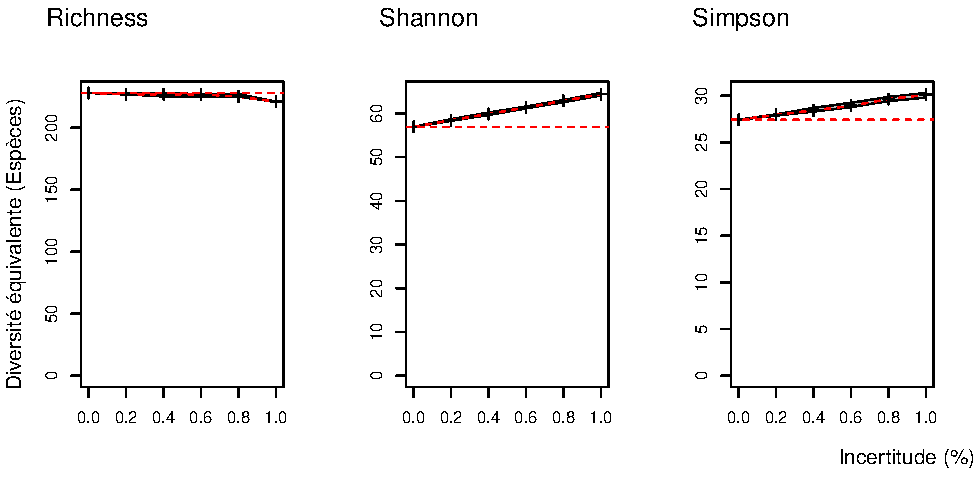
\includegraphics[width=0.6\linewidth]{MyBook_files/figure-latex/FigTreesSp-1} 

}

\caption{Profil de biais pour les diversité de Richesse, Shannon et Simpson au niveau spécifique le long d'un gradient d'indétermination correspondant au pourcentage d'individus identifiés uniquement par leur nom vernaculaire. Les profils de biais représentent la moyenne et les quantiles 0.025 et 0.975 de la distribution des diversités obtenues pour 100 simulations de tirage aléatoire et de propagation des incertitudes.}\label{fig:FigTreesSp}
\end{SCfigure}

Le profil de biais obtenu montre un effet non négligeable du degré
d'indétermination sur la mesure de la diversité. L'estimateur de la
richesse reste peu biaisé tant que le degré d'indétermination ne dépasse
pas 80\%, ce qui signifique que toutes les espèces sont représentées par
au moins un individu identifié au niveau botanique. En revanche les
diversités de Shannon et Simpson, et donc l'équitabilité des
communautés, sont significativement surestimées et ceci
proportionellement au degré d'indétermination.

La propagation des incertitudes tend donc à homogénéiser les abondances
de la communauté: les individus indéterminés tirés aléatoirement ont
plus de chances de orrespondre à une espèce abondante (par définition
plus fréquente) et d'être réattribuée par la méthode de propagation à
une espèce plus commune. Le biais semble donc difficile à formaliser car
il dépend de la relation entre rareté et probabilité d'indétermination
des espèces, qui est déterminée par la connaissances botaniques de
l'équipe d'identification.

Pour pallier ce biais nous avons choisis de nous rapporter au niveau
taxonomique supérieur et d'étudier la diversité des communautés en genre
botanique. Le biais de l'estimateur de diversité au niveau espèce est
bien moins important, ne dépassant pas 10\% de la diversité observée
\ref{fig:FigTreesGenus}. Par ailleurs, les estimateurs sont peu
variables et permettent de comparer correctement les communautés
communautés, pourvu que leurs degrés d'indétermination soient
similaires.

\begin{Shaded}
\begin{Highlighting}[]
\KeywordTok{load}\NormalTok{(}\StringTok{"ExternalFig/Uncertaintypropagation_Species_noCorrection"}\NormalTok{)}

\KeywordTok{par}\NormalTok{(}\DataTypeTok{mfrow=}\KeywordTok{c}\NormalTok{(}\DecValTok{1}\NormalTok{,}\DecValTok{3}\NormalTok{),}\DataTypeTok{no.readonly=}\OtherTok{TRUE}\NormalTok{)}
\KeywordTok{invisible}\NormalTok{(}\KeywordTok{lapply}\NormalTok{(Profile_Genus,}\ControlFlowTok{function}\NormalTok{(ind)\{}
  \KeywordTok{plot}\NormalTok{(}\KeywordTok{colnames}\NormalTok{(ind),ind[}\StringTok{"0.5"}\NormalTok{,],}\DataTypeTok{type=}\StringTok{"n"}\NormalTok{,}\DataTypeTok{ylim=}\KeywordTok{c}\NormalTok{(}\DecValTok{0}\NormalTok{,}\KeywordTok{max}\NormalTok{(ind)),}\DataTypeTok{xlab=}\StringTok{""}\NormalTok{,}\DataTypeTok{ylab=}\StringTok{""}\NormalTok{)}
  \KeywordTok{polygon}\NormalTok{(}\KeywordTok{c}\NormalTok{(}\KeywordTok{colnames}\NormalTok{(ind),}\KeywordTok{rev}\NormalTok{(}\KeywordTok{colnames}\NormalTok{(ind))),}\KeywordTok{c}\NormalTok{(}\KeywordTok{pmax}\NormalTok{(ind[}\StringTok{"0.025"}\NormalTok{,]),}\KeywordTok{pmin}\NormalTok{(}\KeywordTok{rev}\NormalTok{(ind[}\StringTok{"0.975"}\NormalTok{,]))),}\DataTypeTok{col=}\StringTok{"gray75"}\NormalTok{)}
  \KeywordTok{lines}\NormalTok{(}\KeywordTok{colnames}\NormalTok{(ind), ind[}\StringTok{"0.5"}\NormalTok{,], }\DataTypeTok{col =} \StringTok{"red"}\NormalTok{,}\DataTypeTok{lty =} \DecValTok{2}\NormalTok{)}
  \KeywordTok{points}\NormalTok{(}\KeywordTok{colnames}\NormalTok{(ind), ind[}\StringTok{"0.5"}\NormalTok{,], }\DataTypeTok{col =} \StringTok{"black"}\NormalTok{,}\DataTypeTok{pch =} \DecValTok{3}\NormalTok{)}
  \KeywordTok{abline}\NormalTok{(}\DataTypeTok{h=}\NormalTok{ind[}\StringTok{"0.5"}\NormalTok{,}\DecValTok{1}\NormalTok{],}\DataTypeTok{col=}\StringTok{"red"}\NormalTok{,}\DataTypeTok{lty=}\DecValTok{2}\NormalTok{)}
\NormalTok{\}))}
\KeywordTok{mtext}\NormalTok{(}\StringTok{"Incertitude (%)"}\NormalTok{,}\DataTypeTok{side=}\DecValTok{1}\NormalTok{,}\DataTypeTok{cex=}\FloatTok{0.8}\NormalTok{,}\DataTypeTok{outer=}\OtherTok{TRUE}\NormalTok{,}\DataTypeTok{line=}\OperatorTok{-}\DecValTok{2}\NormalTok{,}\DataTypeTok{adj=}\DecValTok{1}\NormalTok{)}
\KeywordTok{mtext}\NormalTok{(}\StringTok{"Diversité équivalente (Genre)"}\NormalTok{,}\DataTypeTok{side=}\DecValTok{2}\NormalTok{,}\DataTypeTok{padj=}\DecValTok{1}\NormalTok{,}\DataTypeTok{cex=}\FloatTok{0.8}\NormalTok{,}\DataTypeTok{line=}\OperatorTok{-}\FloatTok{0.5}\NormalTok{,}\DataTypeTok{outer=}\OtherTok{TRUE}\NormalTok{)}
\KeywordTok{mtext}\NormalTok{(}\StringTok{"Richness"}\NormalTok{,}\DataTypeTok{at=}\FloatTok{0.1}\NormalTok{,}\DataTypeTok{line=}\OperatorTok{-}\FloatTok{1.5}\NormalTok{,}\DataTypeTok{outer=}\OtherTok{TRUE}\NormalTok{);}\KeywordTok{mtext}\NormalTok{(}\StringTok{"Shannon"}\NormalTok{,}\DataTypeTok{at=}\FloatTok{0.44}\NormalTok{,}\DataTypeTok{line=}\OperatorTok{-}\FloatTok{1.5}\NormalTok{,}\DataTypeTok{outer=}\OtherTok{TRUE}\NormalTok{)}
\KeywordTok{mtext}\NormalTok{(}\StringTok{"Simpson"}\NormalTok{,}\DataTypeTok{at=}\FloatTok{0.76}\NormalTok{,}\DataTypeTok{line=}\OperatorTok{-}\FloatTok{1.5}\NormalTok{,}\DataTypeTok{outer=}\OtherTok{TRUE}\NormalTok{)}
\end{Highlighting}
\end{Shaded}

\begin{SCfigure}

{\centering 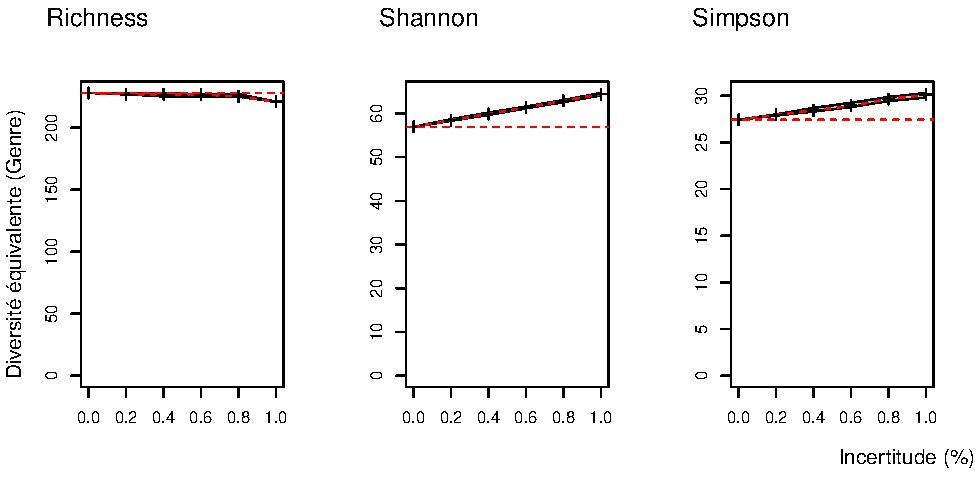
\includegraphics[width=0.6\linewidth]{MyBook_files/figure-latex/FigTreesGenus-1} 

}

\caption{Profil de biais pour les diversité de Richesse, Shannon et Simpson au niveau genre le long d'un gradient d'indétermination correspondant au pourcentage d'individus identifiés uniquement par leur nom vernaculaire. Les profils de biais représentent la moyenne et les quantiles 0.025 et 0.975 de la distribution des diversités obtenues pour 100 simulations de tirage aléatoire et de propagation des incertitudes.}\label{fig:FigTreesGenus}
\end{SCfigure}

\subsection{Cas particulier de
Paracou}\label{cas-particulier-de-paracou}

L'histoire de détermination botanique des parcelles de Paracou implique
une grande variabilité du degré d'indétermination au cours du temps et
des différences significatives entres les parcelles. Aujourd'hui tandis
que les parcelles contrôle et du traitement 3 sont bien déterminées,
moins de 5\% des arbres 'ne sont identifiés que par un nom
vernaculaire'ont pas d'identification botanique, d'autres parcelles du
traitement 1 ou 2 sont encore mal déterminées et pour certaines plus de
30\% des arbres n'ont pas d'identification botanique.

Jusqu'à présent le biais des estimateurs de diversité reste à resoudre,
en revanche il est possible de pallier ces différences de détermination
en considérant la compositon et la diversité des parcelles au niveau du
genre plutôt qu'au niveau de l'espèce.

\chapter{Article 2: trajectoires de diversité des
parcelles}\label{article-2-trajectoires-de-diversite-des-parcelles}

\chapter{Article 3: Dynamiques du
recrutement}\label{article-3-dynamiques-du-recrutement}

\section{Recrutement et mortalité: supports de la dynamique
forestière}\label{recrutement-et-mortalite-supports-de-la-dynamique-forestiere}

La dynamique des peuplement forestiers est la somme des processus
démographiques de mortalité et de recrutement qui régissent l'apparition
(recrutement) et la disparition (mort) des individus dans la communauté.

La disparition d'un arbre, qui libère mécaniquement de l'espace et des
resources, est un processus central de la dynamique forestière. En forêt
tropicale humide en particulier, la mort d'un arbre crée un trou dans la
canopée aux conditions abiotiques nouvelles. On observe alors une
augmentation des radiations lumineuses arrivant au sol, de la
disponibilité en eau et des les flux de chaleur, suivis d'une
augmentation de la productivité du peuplement \autocite[ in Asner
2004]{Pinard2000}. Les trouées augmentent donc la croissance des
individus environnants, des juvéniles ou des plantules de sous-bois et
parfois parfois la germination de graines de la banque du sol. La
mortalité est donc moteur principal de la dynamique forsetière, la
restauration du peuplement après toute perturbation augmentant cette
mortalité dépendra du nombre et de la taille des individus morts
\autocites{Denslow1980}{Schnitzer2001}{Asner2004}.

Le recrutement est le complémentaire de la mortalité pour la dynamique
forestière. Il résulte d'une suite d'événements biologiques depuis la
production, la dissémination et la germination des graines, à la survie
et la croissance des plantule jusqu'au seuil de recrutement. Ce seuil de
recrutement correspond souvent à un diamètre minimum, représentatif de
la taille et de la biomasse de l'arbre, à partir duquel on considère
l'individu assez développé pour avoir un rôle significatif au sein du
peuplement. L'écologie des espèces détermine en effet les conditions
nécessaires à la germination, la croissance et la survie des individus:
filtres environnementaux et exclusions compétitives s'opèrent donc
s'exercent donc principalement au cours du recrutement. Le recrutement
est donc le deuxième élément essentiel régissant la composition et la
diversité des communautés en forêt tropicale et permet de plus
d'appréhender le futur des forêts tropicales en en définissant le
peuplement en devenir \autocite[ + cf biblio Elodie]{Denslow1980}.

\chapter{Conclusion et perspectives}\label{conclusion-et-perspectives}


% Bibliography
%%%%%%%%%%%%%%%%%%%%%%%%%%%%%%%%%%%%%%%%%%%%%%%%%%%%%%%%%%

\backmatter
\SmallMargins

%
\printbibliography


% Tables (of tables, of figures)
%%%%%%%%%%%%%%%%%%%%%%%%%%%%%%%%%%%%%%%%%%%%%%%%%%%%%%%%%%




% After-body (LaTeX code inclusion)
%%%%%%%%%%%%%%%%%%%%%%%%%%%%%%%%%%%%%%%%%%%%%%%%%%%%%%%%%%



% Back cover
%%%%%%%%%%%%%%%%%%%%%%%%%%%%%%%%%%%%%%%%%%%%%%%%%%%%%%%%%%%

% Even page, small margins, no running head, no page number.
\evenpage
\SmallMargins
\thispagestyle{empty}

\begin{normalsize}

\begin{description}

\selectlanguage{french}
\item[Résumé:]
A venir

\selectlanguage{french}
\item[Mots clés :]
Biodiversité, Forêts Néotropicales, Perturbation, Ecologie des Communautés, Dynamique.
~\\

\selectlanguage{english}
\item[Abstract:]
To be coming

\selectlanguage{english}
\item[Keywords:]
Biodiversity, Neotropical forests, Perturbation, Communities Ecology, Dynamic.

\end{description}

\end{normalsize}

\vspace*{\fill}
\centering\includegraphics[width=.3\textwidth]{images/Logo-Lab}
\end{document}
